At the end of last section, we stated that information from ganglion cells extend to the Lateral Geniculate Nucleus (LGN), where information is relayed and organized so that the cortex can interpret it. Organization makes left visual field sent to right hemisphere, right field to left hemisphere (Figure~\ref{fig:vision:optic-chiasm}).

\begin{figure}
  \begin{center}
    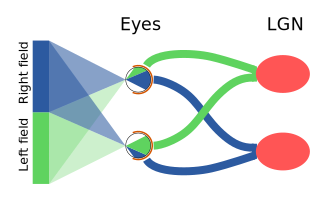
\includegraphics[width=0.7\textwidth]{visual-fields-lgn}
    \caption{Visual field mapping in LGN.}
    \label{fig:vision:optic-chiasm}
  \end{center}
\end{figure}

The portion of the cortex that is involved with visual processing has been estimated to about 30\%.

It has been studied and areas have been labelled due to their function.

V1, V2, V...

